\section{Аналитическая часть}

\subsection{Организация приема в вузы России}

В настоящее время, набор на программы подготовки специалистов и бакалавров в российские ВУЗы проводится по результатам Единого Государственного Экзамена\cite{ege}, который должны сдавать все школьники по окончании 11 классов общеобразовательного учреждения, причем для получения аттестата необходимо сдать как минимум 2 обязательных предмета: русский язык и математику. До 2021 года прием в вузы проводился по результатам трех (иногда четырех) ЕГЭ, определенных для каждой специальности. Все абитуриенты российских университетов должны были предоставить в приемную комиссию результаты ЕГЭ по русскому языку и профильному ЕГЭ по выбранной специальности, третий предмет ВУЗ выбирал самостоятельно из перечня экзаменов, определенных для данного направления. С 2022 года учебные заведения вправе установить третий ЕГЭ на выбор абитуриента из нескольких предложенных вариантов. Для того, чтобы подать документы в выбранный ВУЗ, необходимо набрать на ЕГЭ по каждому предмету количество баллов, равное или превышающее минимальный балл. ВУЗ сам определяет минимальный балл для каждой специальности и направления, но не может установить его ниже уровня, утвержденного Рособрнадзором\cite{prikaz}.

Каждый выпускник имеет право одновременно подать документы в 5 ВУЗов, в каждом можно выбрать 1-10 специальностей по всем формам обучения. Количество специальностей с 2021 года определяется ВУЗом. Схематично это представлено на рисунке \ref{five-vuzov}.

\begin{figure}[hbtp]
	\centering
	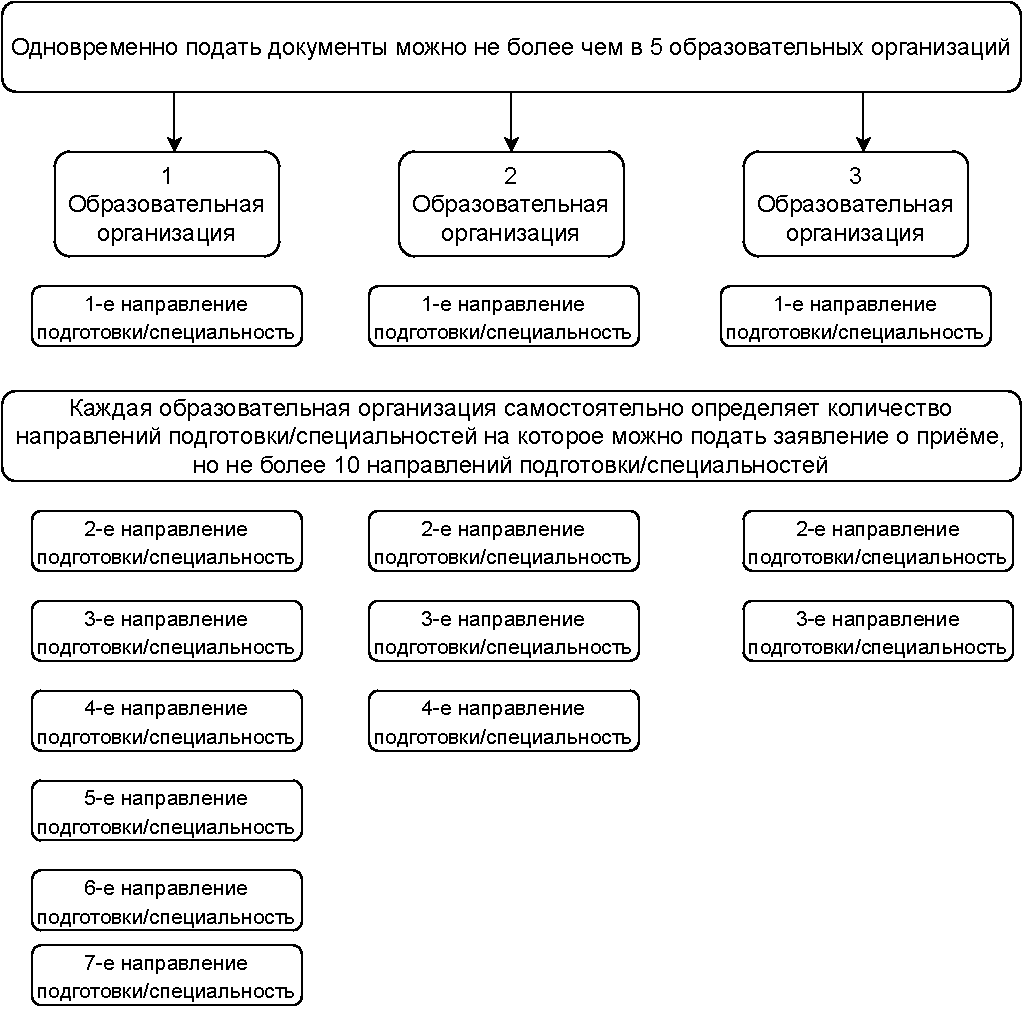
\includegraphics[scale=0.8]{img/fivevuzov.drawio.pdf}
	\caption{Подача заявления возможна не более чем в 5 образовательных учреждений}
	\label{five-vuzov}
\end{figure}

Списки абитуриентов, подавших документы, ранжируются по количеству баллов, то есть более высокие позиции занимают абитуриенты, у которых совокупное количество баллов за ЕГЭ, дополнительные вступительные испытания и индивидуальные достижения выше. Рассматривается сумма баллов без учета индивидуальных достижений, затем профильный предмет и далее в порядке убывания приоритетности. Если у двух абитуриентов совпадает весь перечень, то приоритет отдается тому, у кого есть преимущественное право. При равенстве по всем критериям список ранжируется по индивидуальным достижениям, учитываемым при равенстве поступающих по иным критериям ранжирования. В таблице \ref{list:abitur} представлен простой ранжированный список поступающих.

\begin{table}[!hbp]
	\caption{\label{list:abitur}Ранжированный список поступающих.}
	\begin{center}
		\begin{tabular}{|l|l|l|l|l|}
			\hline
			Номер в сводке & Фамилия & Балл & Наличие аттестата & Наличие заявления \\
			\hline
			1 & Гусев & 299 & Нет &  Нет \\
			\hline
			2 & Слепухина & 282 & Нет &  Нет \\
			\hline
			3 & Стрельцов & 265 & Нет &  Да \\
			\hline
			4 & Абасов & 248 & Да &  Да \\
			\hline
			5 & Петрова & 221 & Нет &  Нет \\
			\hline
			6 & Калинин & 201 & Да &  Нет \\
			\hline
			7 & Иванов & 194 & Да &  Да \\
			\hline
		\end{tabular}
	\end{center}
\end{table}

Согласно правилам приема\cite{porydok}, ВУЗы к результатам ЕГЭ могут добавить своим абитуриентам до 10 баллов за индивидуальные достижения. Каждый университет сам устанавливает количество дополнительных баллов за индивидуальные достижения. Как правило, больше всего баллов университеты добавляют за аттестат с отличием и результаты олимпиад, не использованные для получения особых прав.

После этого начинается зачисление. До 2021 года оно проходило в несколько этапов:

\begin{itemize}[leftmargin=1.6\parindent]
	\item этап приоритетного зачисления — зачисляют абитуриентов, которые поступают без экзаменов, в рамках особой или целевой квоты\cite{celevoi}. Эти абитуриенты должны подать в ВУЗ оригинал документа о предшествующем образовании и заявление о согласии на зачисление;
	\item I этап зачисления — на этом этапе ВУЗ может заполнить до 80\% бюджетных мест, оставшихся свободными после приоритетного зачисления, по каждой специальности или направлению. Абитуриентов зачисляют в соответствии с позицией, которую они занимают в списке поступающих, — первыми зачисляют тех, кто занимает более высокую позицию. На этом этапе нужно подать оригинал документа о предшествующем образовании и заявление о согласии на зачисление;
	\item II этап зачисления — вуз заполняет оставшиеся 20\% бюджетных мест.

\end{itemize}

 С 2021 года основная волна зачисления только одна\cite{prikaz1}. На досрочном этапе ВУЗы принимают олимпиадников, поступающих вне конкурса, абитуриентов, имеющих льготы, и целевиков. Если после основной волны останутся свободные места, ВУЗ вправе принять на них абитуриентов из конкурсного списка.

По итогам конкурса определяется проходной балл — наименьшее количество баллов, которого оказалось достаточно для зачисления. Таким образом, проходной балл меняется каждый год и определяется только после зачисления. Абитуриенты, которые поступают по квотам, имеют право принимать участие и в общем конкурсе. Для этого они также должны набрать количество баллов, равное или превышающее минимальное значение, установленное ВУЗом.

\subsection{Статистические данные}

Согласно статистике на 2019 год, в России ведёт образовательную деятельность 741 государственный ВУЗ \cite{stat}. Публичную информацию о них можно получить на следующих ресурсах:

\begin{itemize}[leftmargin=1.6\parindent]
	\item мониторинг качества приема в ВУЗы\cite{hse};
	\item информационно-аналитические материалы по результатам проведения мониторинга
эффективности деятельности образовательных организаций высшего образования\cite{miccedu}.

\end{itemize}

В таблице \ref{list:hseinfo} приведен пример получаемой информации с первого ресурса по направлениям подготовки.

\begin{table}[]
	\caption{\label{list:hseinfo}Пример информации по направлениям подготовки.}
\begin{tabular}{|c|c|c|c|c|}
\hline
\begin{tabular}[c]{@{}c@{}}Название\\ ВУЗа\end{tabular}        & \begin{tabular}[c]{@{}c@{}}Направление\\ подготовки\end{tabular} & Год  & \begin{tabular}[c]{@{}c@{}}Средний балл ЕГЭ\\ поступивших на\\ бюджетные места\end{tabular} & \begin{tabular}[c]{@{}c@{}}Число студентов, \\ поступивших на \\ бюджетные места\end{tabular} \\ \hline
\begin{tabular}[c]{@{}c@{}}Орловский\\  гос. ун-т\end{tabular} & Биология                                                         & 2020 & 59.9                                                                                        & 46                                                                                            \\ \hline
\end{tabular}
\end{table}

Из информационного-аналитических материалов второго ресурса можно получить обширную статистику по многим показателям вуза, выделим основные из них:

\begin{itemize}[leftmargin=1.6\parindent]
	\item название ВУЗа;
	\item регион расположения учреждения;
	\item год статистики;
	\item наличие общежития;
	\item средний балл ЕГЭ по очной форме на бюджетные места;
	\item средний балл ЕГЭ по очной форме на бюджетные места по общему конкурсу;
	\item усредненный по реализуемым направлениям минимальный балл ЕГЭ по очной форме на программы бакалавриата и специалитета;
	\item численность студентов, победителей и призеров заключительного этапа всероссийской олимпиады школьников, членов сборных команд Российской Федерации принятых на очную форму обучения на первый курс по программам бакалавриата и специалитета без вступительных испытаний;
	\item численность студентов, победителей и призеров олимпиад школьников, принятых на очную форму обучения на первый курс по программам бакалавриата и специалитета;
	\item численность студентов, принятых по результатам целевого приема на первый курс на очную форму обучения по программам бакалавриата и специалитета;
	\item удельный вес численности студентов, принятых по результатам целевого приема на первый курс на очную форму обучения по программам бакалавриата и специалитета в общей численности студентов, принятых на первый курс по программам бакалавриата и специалитета на очную форму обучения;
	\item удельный вес численности иностранных студентов (кроме стран Содружества Независимых Государств), обучающихся программам бакалавриата, специалитета, магистратуры, в общей численности студентов (приведенный контингент);
	\item удельный вес численности иностранных студентов из СНГ, обучающихся по программам бакалавриата, специалитета, магистратуры, в общей численности студентов (приведенный контингент);
	\item средний балл ЕГЭ студентов, принятых на обучение по программам бакалавриата и специалитета, по всем формам обучения;
	\item доля обучающихся по программам бакалавриата, специалитета, магистратуры в очной форме;
	\item список реализуемых УГСН.
\end{itemize}

Статистические данные о распределении абитуриентов по регионам, количестве 100-бальников в каждом из них России можно получить на портале открытых данных \cite{egestat}.

Перечень вступительных испытаний при приеме на обучение по образовательным
программам высшего образования - программам бакалавриата и программам специалитета можно получить из приказа Минобрнауки России \cite{prikaz2}.

\subsection{Построение устойчивых паросочетаний}

Исследование механизмов построения паросочетаний в ситуациях, когда участники имеют предпочтения и свободу принятия решений, было начато в классической работе\cite{gale}. Авторы рассматривали модели построения паросочетаний один-к-одному (когда каждый участник получает не более одного партнера) и один-ко-многим (когда участник одной стороны рынка – студенты получают ровно одного партнера, а
участники другой стороны рынка – ВУЗы получают более одного
партнера). Авторами был предложен алгоритм, позволяющий за конечное число шагов получить паросочетание при известных предпочтениях
участников, являющихся линейными порядками на множестве участников противоположной стороны. В литературе этот алгоритм называется алгоритмом отложенного принятия (deffered acceptance algorithm).

Существует две версии алгоритма в зависимости от того, кто является
предлагающей стороной, абитуриенты или ВУЗы.
Рассмотрим вариант, в котором предлагающей стороной являются студенты. До начала работы алгоритма подаются предпочтения участников – линейные порядки на множестве агентов противоположной стороны.
На первом шаге каждый абитуриент обращается в наиболее предпочтительный для себя ВУЗ. ВУЗ рассматривает все полученные заявления и временно принимает q лучших абитуриентов, где q соответствует числу мест. На следующем шаге те абитуриенты, которым было отказано,
обращаются в следующие по предпочтительности ВУЗы, они снова
рассматривают все полученные заявления (оставленные с первого шага
и вновь поступившие). Если ВУЗ получает новое заявление от абитуриента, которого он предпочтитает временно зачисленному, то последнему
ВУЗ отказывает и на следующем шаге такой абитуриент делает предложение следующему ВУЗу. Эта процедура продолжается до тех пор,
пока все абитуриенты не будут зачислены в ВУЗы либо не получат отказ от всех ВУЗов, указанных в предпочтениях.
Важным достоинством механизма является то, что он позволяет получить устойчивое паросочетание, то есть такое, что

\begin{itemize}[leftmargin=1.6\parindent]
	\item никакой участник не хочет отказаться от предложенного партнера и остаться один;
	\item никакие два участника не желают сговориться и заключить соглашение 
друг с другом, избежав предписанного распределения.
\end{itemize}

Кроме того, при использовании варианта механизма, в котором предлагающей стороной являются студенты, им оказывается выгодно представлять свои истинные предпочтения. Работа\cite{gale} получила широкое развитие и в теоретических исследованиях, и в прикладном дизайне централизованных механизмов. Механизм
отложенного принятия (с незначительными вариациями) был внедрен
на программе распределения медицинских интернов в США, системе
зачисления в ВУЗы Турции по итогам единого тестирования, а также
в департаментах образования Бостона, Нью-Йорка и других городов
США для зачисления в муниципальные школы.

\subsection{Бостонский механизм построения неустойчивых паросочетаний}

Описанный механизм часто именуется "Бостонским механизмом" так как именно этот механизм использовался для распределения детей Бостона по муниципальным школам.

Перед началом работы механизма участники (школы и поступающие)
сообщают свои предпочтения в виде линейных порядков (списков) друг
относительно друга. На первом шаге каждый абитуриент подает заявку
в наилучшую для себя школу. Если школа получила больше заявок, чем
имеется мест, то она отбирает лучших абитуриентов. На втором шаге
абитуриенты, отвергнутые на первом шаге, подают заявки во вторые по
предпочтительности школы. Школы не пересматривают результаты зачисления на первом шаге, даже если вновь обратившиеся абитуриенты
для них предпочтительнее уже зачисленных. Каждая школа зачисляет
лучших из вновь обратившихся абитуриентов на оставшиеся места. Так
продолжается до тех пор, пока все абитуриенты не будут зачислены
(либо отвергнуты всеми школами).
Такой механизм ведет к созданию неустойчивого паросочетания. Действительно, рассмотрим абитуриента, поставившего на первое и второе
места школы X и Y, соответственно. Пусть на первом шаге школа X не
приняла абитуриента, так как получила достаточное количество заявлений
от более предпочтительных абитуриентов; школа Y также полностью
заполнила свои места на первом шаге. Тогда на втором шаге абитуриент
подает заявление в Y. Но даже если Y считает этого абитуриента лучшим среди всех, она не сможет его принять, так как все места заполнены
на первом шаге.


Этот алгоритм был заменен алгоритмом отложенного принятия, что позволило улучшить
получаемое распределение для существенной доли абитуриентов и ликвидировать необходимость манипулирования при представлении предпочтений.


\subsection{Агентно-ориентированное моделирование}

Агентное моделирование – это мощный метод имитационного моделирования, который за последние несколько лет нашел применение в ряде прикладных задач, таких как потребительские и финансовые рынки, организационное поведение, транспортные системы, логистика.

Агентно-ориентированное моделирование – это система которая моделируется как совокупность автономных субъектов принятия решений, называемых агентами.
Каждый агент индивидуально оценивает свою ситуацию и принимает решения на основе набора правил. Агенты могут демонстрировать различное поведение,
подходящее для системы, которую они представляют, например, производство, потребление или продажа. На простейшем уровне агент-ориентированная модель состоит из системы агентов и отношений между ними. Даже простая агентно-ориентированная модель может демонстрировать сложные модели поведения и предоставлять ценную информацию о динамике реальной системы, которую она имитирует. 
Агент – некоторая сущность обладающая активностью, некоторой активностью поведения. Может принимать решение в соответствии с некоторым набором правил взаимодействия с окружением, а также самостоятельно изменяться. Кроме того, агенты могут развиваться, позволяя проявиться непредвиденному поведению. Сложная система иногда включает нейронные сети, эволюционные алгоритмы или другие методы обучения, чтобы обеспечить реалистичное обучение и адаптацию.

\subsubsection{Структура агентно-ориентированной модели}

Типичная агентная модель состоит из трех элементов:

\begin{itemize}[leftmargin=1.6\parindent]
	\item[---] набор агентов, их атрибуты и поведение;
	\item[---] набор агентских отношений и способов взаимодействия;
	\item[---] среда агентов, где они взаимодействуют между собой.

\end{itemize}

\begin{figure}[hbtp]
	\centering
	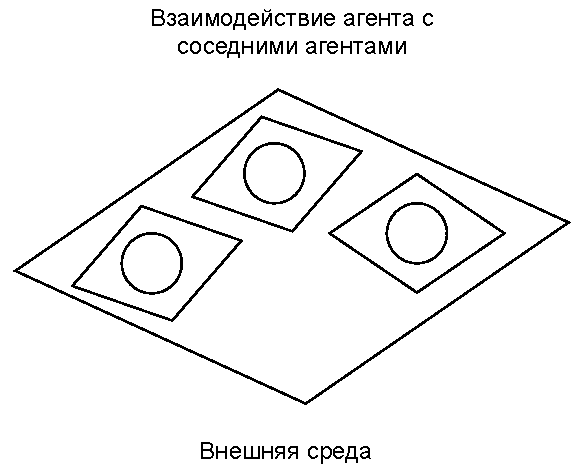
\includegraphics[scale=0.8]{img/typical-model.drawio.pdf}
	\caption{Структура типичной агентно-ориентированной модели}
	\label{typical-model}
\end{figure}

Для создания модели на основе агентов необходимо проанализировать, смоделировать и запрограммировать эти элементы. 

Структура типичной модели показана на рисунке \ref{typical-model}. Каждый элемент данной структуры будет разобран далее.

\subsubsection{Агент как элемент структуры модели}

Наиболее важная определяющая характеристика агента – это его способность действовать автономно, то есть действовать самостоятельно в ответ на ситуации, с которыми он сталкивается. Агенты наделены поведением, которое позволяет им принимать независимые решения, обычно они активны, инициируют свои действия для достижения внутренних целей, а не просто пассивны, реагируют на других агентов и окружающую среду.

С точки зрения практического моделирования, агенты обладают некоторыми существенными характеристиками:

\begin{itemize}[leftmargin=1.6\parindent]
	\item 	автономность и однозначная идентифицируемость;
	\item самостоятельность, может независимо функционировать в своей среде и взаимодействовать с другими агентами, по крайней мере, в ограниченном диапазоне ситуаций, представляющих интерес для модели;
	\item агент имеет состояние, которое представляет основные переменные, связанные с его текущей ситуацией;
	\item динамичное взаимодействие с другими агентами, влияющими на его поведение. У агентов есть протоколы для взаимодействия с другими агентами, способность реагировать на окружающую среду. 

\end{itemize}

\begin{figure}[hbtp]
	\centering
	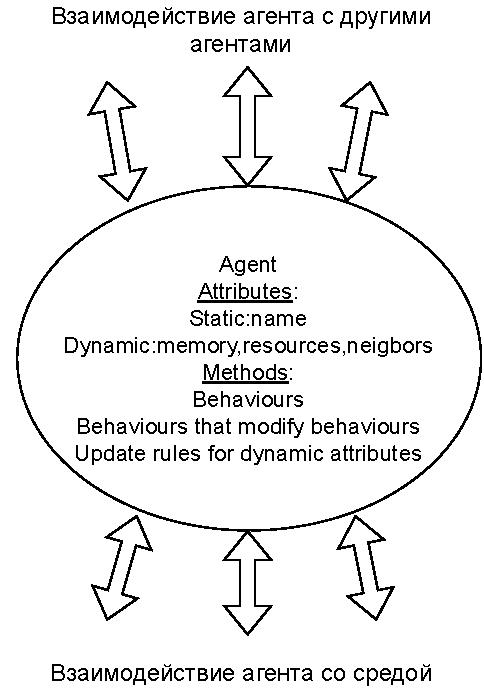
\includegraphics[scale=0.8]{img/typical-agent.drawio.pdf}
	\caption{Структура типичного агента}
	\label{typical-agent}
\end{figure}

Структура типичного агента показана на рисунке \ref{typical-agent}.  Все связанное с агентом является атрибутом, либо методом, который работает с агентом. Атрибуты могут быть статическими, не изменяемыми во время моделирования, и динамическими. Например, статический атрибут – это имя агента, динамический атрибут - это память агента о прошлых взаимодействиях.


\subsubsection{Взаимодействие агентов}

Двумя основными проблемами моделирования взаимодействий агентов являются определение того, кто с кем может быть связан, и механизмы динамики взаимодействий. Оба аспекта необходимо учитывать при разработке агентно-ориентированных моделей. Один из принципов сложных систем и агентного моделирования заключается в том, что агенту доступна только локальная информация. Агентные системы – это децентрализованные системы, нет центрального органа, который либо распространяет глобально доступную информацию всем агентам, либо контролирует их поведение в целях оптимизации производительности системы. Агенты взаимодействуют с другими агентами, но не все постоянно взаимодействуют напрямую со остальными, как в реальных системах. Агенты обычно взаимодействуют с подмножеством других агентов, называемых соседями. Локальная информация получается из взаимодействий с соседями агента (не с каким-либо агентом или всеми агентами) и из его локальной среды (а не из какой-либо части всей среды). Как правило, набор соседей агента быстро меняется по мере моделирования. То, как агенты связаны друг с другом, обычно называют топологией или связностью агентно-ориентированной модели. Типичные топологии включают пространственную сетку или сеть узлов (агентов) и связей (отношений).

\subsection{Формализация задачи}

В соответствии с выбранной темой выпускной квалификационной работы необходимо разработать и реализовать метод прогнозирования итогов
приёма в ВУЗы России на основе агентного моделирования с использованием полученных из открытых источников статистических данных о ВУЗах и УГСН, а также распределении абитуриентов по регионам. Необходимо провести обработку полученных статистических данных. 

Входные данные для проведения моделирования:

\begin{itemize}[leftmargin=1.6\parindent]
	\item[---] статистические данные о ВУЗах и их УГСН;
	\item[---] распределение абитуриентов по регионам России;
	\item[---] перечень вступительных испытаний и соответствующие ему УГСН;
	\item[---] популяция агентов (абитуриентов) с заданными характеристиками.

\end{itemize}

Результатом проведенного моделирования являются:

\begin{itemize}[leftmargin=1.6\parindent]
	\item[---] средний балл зачисленных абитуриентов по каждому ВУЗу, участвовавшему в моделировании;
	\item[---] максимальный балл по каждому ВУЗу;
	\item[---] минимальный балл по каждому ВУЗу;
	\item[---] количество зачисленных абитуриентов по каждому ВУЗу;
	\item[---] средний балл всех зачисленных абитуриентов на конкретный УГСН по каждому ВУЗу;
	\item[---] максимальный балл по каждому УГСН;
	\item[---] минимальный балл по каждому УГСН;
	\item[---] количество зачисленных абитуриентов по каждому УГСН.

\end{itemize}

Для всех значений баллов в результатах моделирования необходимо показать изменение (в количественном выражении) в сравнении с результатом приема прошлого года.















\pagebreak